% Options for packages loaded elsewhere
\PassOptionsToPackage{unicode}{hyperref}
\PassOptionsToPackage{hyphens}{url}
%
\documentclass[
]{article}
\usepackage{amsmath,amssymb}
\usepackage{lmodern}
\usepackage{iftex}
\ifPDFTeX
  \usepackage[T1]{fontenc}
  \usepackage[utf8]{inputenc}
  \usepackage{textcomp} % provide euro and other symbols
\else % if luatex or xetex
  \usepackage{unicode-math}
  \defaultfontfeatures{Scale=MatchLowercase}
  \defaultfontfeatures[\rmfamily]{Ligatures=TeX,Scale=1}
\fi
% Use upquote if available, for straight quotes in verbatim environments
\IfFileExists{upquote.sty}{\usepackage{upquote}}{}
\IfFileExists{microtype.sty}{% use microtype if available
  \usepackage[]{microtype}
  \UseMicrotypeSet[protrusion]{basicmath} % disable protrusion for tt fonts
}{}
\makeatletter
\@ifundefined{KOMAClassName}{% if non-KOMA class
  \IfFileExists{parskip.sty}{%
    \usepackage{parskip}
  }{% else
    \setlength{\parindent}{0pt}
    \setlength{\parskip}{6pt plus 2pt minus 1pt}}
}{% if KOMA class
  \KOMAoptions{parskip=half}}
\makeatother
\usepackage{xcolor}
\IfFileExists{xurl.sty}{\usepackage{xurl}}{} % add URL line breaks if available
\IfFileExists{bookmark.sty}{\usepackage{bookmark}}{\usepackage{hyperref}}
\hypersetup{
  pdftitle={Jabbing Together?},
  pdfauthor={Byron Carson, Justin Isaacs, and Tony Carilli},
  hidelinks,
  pdfcreator={LaTeX via pandoc}}
\urlstyle{same} % disable monospaced font for URLs
\usepackage[margin=1in]{geometry}
\usepackage{longtable,booktabs,array}
\usepackage{calc} % for calculating minipage widths
% Correct order of tables after \paragraph or \subparagraph
\usepackage{etoolbox}
\makeatletter
\patchcmd\longtable{\par}{\if@noskipsec\mbox{}\fi\par}{}{}
\makeatother
% Allow footnotes in longtable head/foot
\IfFileExists{footnotehyper.sty}{\usepackage{footnotehyper}}{\usepackage{footnote}}
\makesavenoteenv{longtable}
\usepackage{graphicx}
\makeatletter
\def\maxwidth{\ifdim\Gin@nat@width>\linewidth\linewidth\else\Gin@nat@width\fi}
\def\maxheight{\ifdim\Gin@nat@height>\textheight\textheight\else\Gin@nat@height\fi}
\makeatother
% Scale images if necessary, so that they will not overflow the page
% margins by default, and it is still possible to overwrite the defaults
% using explicit options in \includegraphics[width, height, ...]{}
\setkeys{Gin}{width=\maxwidth,height=\maxheight,keepaspectratio}
% Set default figure placement to htbp
\makeatletter
\def\fps@figure{htbp}
\makeatother
\setlength{\emergencystretch}{3em} % prevent overfull lines
\providecommand{\tightlist}{%
  \setlength{\itemsep}{0pt}\setlength{\parskip}{0pt}}
\setcounter{secnumdepth}{-\maxdimen} % remove section numbering
\newlength{\cslhangindent}
\setlength{\cslhangindent}{1.5em}
\newlength{\csllabelwidth}
\setlength{\csllabelwidth}{3em}
\newlength{\cslentryspacingunit} % times entry-spacing
\setlength{\cslentryspacingunit}{\parskip}
\newenvironment{CSLReferences}[2] % #1 hanging-ident, #2 entry spacing
 {% don't indent paragraphs
  \setlength{\parindent}{0pt}
  % turn on hanging indent if param 1 is 1
  \ifodd #1
  \let\oldpar\par
  \def\par{\hangindent=\cslhangindent\oldpar}
  \fi
  % set entry spacing
  \setlength{\parskip}{#2\cslentryspacingunit}
 }%
 {}
\usepackage{calc}
\newcommand{\CSLBlock}[1]{#1\hfill\break}
\newcommand{\CSLLeftMargin}[1]{\parbox[t]{\csllabelwidth}{#1}}
\newcommand{\CSLRightInline}[1]{\parbox[t]{\linewidth - \csllabelwidth}{#1}\break}
\newcommand{\CSLIndent}[1]{\hspace{\cslhangindent}#1}
\usepackage{setspace}
\doublespacing
\usepackage{lineno}
\linenumbers
\ifLuaTeX
  \usepackage{selnolig}  % disable illegal ligatures
\fi

\title{Jabbing Together?}
\usepackage{etoolbox}
\makeatletter
\providecommand{\subtitle}[1]{% add subtitle to \maketitle
  \apptocmd{\@title}{\par {\large #1 \par}}{}{}
}
\makeatother
\subtitle{The Complementarity Between Social Capital, Formal Public
Health Rules, and COVID-19 Vaccine Rates in the United States}
\author{Byron Carson, Justin Isaacs, and Tony Carilli}
\date{}

\begin{document}
\maketitle
\begin{abstract}
COVID-19 vaccine rates provide a unique opportunity to explore vaccine
hesitancy and potential interactions between social capital and
individual, normative values, namely for public health and/or personal
freedom. While economists and public health scholars realize the
independent effects social capital and stringent public health rules
have on prevalence and mortality rates, few recognize how these factors
influence vaccination rates. We advance this literature with a novel
framework to analyze these interactions. With county-level data on
COVID-19 vaccinations, social capital, and measures of the values people
have for personal freedom and public health, we find that vaccination
rates depend on individual values, the level of social capital, and the
interaction between the two. Social capital mediates the values people
hold dear, which can influence vaccination rates in positive and
negative ways. Our results are robust to the inclusion of relevant
controls and under multiple specifications. These results suggest that
individuals and the communities people enter into and exit out of play
an important role in decisions to vaccinate, which are independent of
formal, governmental public health measures.
\end{abstract}

\newpage

\hypertarget{introduction}{%
\section{Introduction}\label{introduction}}

Vaccine hesitancy---among parents, among healthcare professional, and
for particular diseases---is an on-going public health concern
(MacDonald and SAGE Working Group on Vaccine Hesitancy 2015). As useful
as vaccines are, people eschew them because of religious values,
perceptions of vaccine inefficacy, vaccine campaigns of the past that
used coercion and/or fraud (Dubé et al. 2013; Ozawa and Stack 2013;
Yaqub et al. 2014; Karafillakis et al. 2016; Cadeddu et al. 2021). While
there are various definitions of vaccine hesitancy, there is no single
set of factors that consistently explains differences in hesitancy or
identifies policies to improve hesitancy (Larson et al. 2014; Eskola et
al. 2015).\footnote{Vaccine hesitancy is ``A behaviour, influenced by a
  number of factors including issues of confidence {[}do not trust a
  vaccine or provider{]}, complacency {[}do not perceive a need for a
  vaccine, do not value the vaccine{]}, and convenience {[}access{]}''
  (Larson et al. 2014: 2151).}

Vaccine hesitancy becomes more pressing as we consider COVID-19
vaccination and especially relevant for minority populations who might
face additional health burdens (Hildreth and Alcendor 2021; Khubchandani
and Macias 2021). As it relates to COVID-19 vaccination, few studies
indicate consistent factors of hesitancy. For example, Christian
Nationalism is correlated with hesitancy (Corcoran, Scheitle, and
DiGregorio 2021), as are socio-economic and education variables (Mollalo
and Tatar 2021; Lazarus et al. 2020). Hesitancy also remains high in
high-income countries, especially among younger, poorer, female,
non-White, and less educated groups (Aw et al. 2021). Similarly, Hudson
and Montelpare (2021) shows that while age, income, education, parental
status, rurality, trust in authority, disgust sensitivity, and risk
aversion can explain COVID-19 vaccination rates, these results are
tentative given the lack of peer-review and the novelty of our
experiences with COVID-19 vaccination. Moreover, studies that rely on
theories of planned behavior consistently explain differences in
hesitancy (Xiao and Wong 2020).

A related strand of public health research explores the role social
capital---a kind of informal, social norm---plays in vaccination,
disease prevention, and health promotion (see, for example, Putnam
2001). As it relates to vaccinations, higher levels of social capital
lead to higher rates of second-round measles vaccinations (Nawa and
Fujiwara 2019; Nagaoka, Fujiwara, and Ito 2012). Similarly, social
capital influences vaccines for pneumonia among elderly populations in
Japan (Iwai-Saito, Shobugawa, and Kondo 2021). Various measures of
social capital also influence influenza vaccine rates in Taiwan (Chuang
et al. 2015), and with H1N1 in Scandinavia (Björn Rönnerstrand 2013; B.
Rönnerstrand 2014) (also, see Jung, Lin, and Viswanath 2013).

There is a growing consensus in public discourse and in scholarly work
that social capital leads to good public health outcomes in the context
of COVID-19 (Gopnik 2020; Imbulana Arachchi and Managi 2021; Pitas and
Ehmer 2020; Wong and Kohler 2020; Borgonovi, Andrieu, and Subramanian
2021; Dutta, Makridis, and Rao 2021). At the county level in the U.S.
between March and July of 2020, for example, Makridis and Wu (2021)
isolate the effect social capital and its components have on rates of
COVID-19 prevalence and mortality with standard empirical techniques,
e.g., fixed effects that might attenuate omitted variable bias and
alternative measures of social capital. They report that the spread of
COVID-19 falls by 18 percent (and deaths fall by 5.7 percent) as
counties increase their social capital from the 25th percentile to the
75th percentile. Ferwana and Varshney (2021) shows that different
components of social capital have differing effects.

We suggest, however, that social capital does not unambiguously confer
positive public health outcomes. Social capital reinforces the
subjective values people have. For instance, social capital might
encourage the use of interpersonal networks to care for one another and
provide support from a distance, but it can also reinforce beliefs
within a community that prioritize personal freedom over public health.
Following Carson, Isaacs, and Carilli (2021) and their framework on the
interactions between individual values, formal public health rules, and
social capital, we develop a framework to 1) assess the conditions under
which social capital influences the magnitude of vaccination, and 2)
compare the effects social capital has on vaccination relative to a
community's taste for public health versus personal freedom.

With over one year's worth of county-level, daily data on COVID-19
vaccination rates, social capital, and regulatory stringency in the
United States, we build a county-level, cross-sectional model to assess
these relative effects. Our main result is that counties with stronger
social capital (relative to the average) and higher values for public
health namely COVID-19 prevention (relative to the average) are less
hesitant to use vaccines. We also find that social capital reinforces
beliefs of personal freedom, which increases hesitancy and a lower level
of vaccination where those values are prevalent. Our results are robust
across measured sub-components of social capital, to the inclusion of
standard controls, and alternative measures of social capital. These
results suggest that the values people have, their formal and informal
rules, and their interactions play identifiable roles in the use of
vaccines as a preventative measure in the fight against the spread of
COVID-19.

\hypertarget{values-social-capital-and-covid-19}{%
\section{Values, Social Capital, and
COVID-19}\label{values-social-capital-and-covid-19}}

Social capital encourages people to trust each other, which encourages
various kinds of cooperation and even private health outcomes. People
with greater social capital might have more financial resources, e.g.,
charity; they might have greater access to organizations that lower the
cost of health care; they might be constrained by social norms that
influence health; and they might have a greater ability to engage in
political action (Putnam 2001).

We argue that social capital complements or reinforces the underlying
normative values people have for prevention and the subsequent actions
they adopt, e.g., personal responses, public health rules, mandates, and
vaccine use. We expect people to increase the magnitude of vaccination
when 1) they place a higher value on prevention and 2) they have a
higher level of social capital that reinforces such values, behaviors,
and rules. While social capital reinforces preventative behaviors and
vaccination in areas that value prevention, it can reinforce infectious
behaviors in areas that value personal freedom. Our framework indicates
the possibility of both positive and negative public health outcomes.
That is, areas can experience a higher level of vaccination because of
their general appreciation for public health over personal freedom and
their higher level of social capital. At the same time, areas can
experience a lower level of vaccination because of their general
appreciation for personal freedom over public health and their higher
level of social capital. Thus, the interaction between social capital
and how people value public health over personal freedom become
important determinants of the formal rules people favor and their
vaccination behaviors.

We suggest the interaction between social capital, values for
prevention, and formal rules influences the magnitude of vaccination
because social capital raises the private costs to individuals of
breaking the rules that a group perceives as legitimate, namely formal
and informal public health rules. People with stronger levels of social
capital are more likely to interact with each other---which can increase
the spread of diseases like COVID-19---but they are also likely to
follow public health suggestions and mandates they value (Carson,
Isaacs, and Carilli 2021). The more people value disease prevention over
other legitimate values like personal freedom, and the more they believe
public health claims are also legitimate and valuable, breaking those
rules is taken as an affront punishable informally by a personal rebuke,
a worsening reputation, a refusal of service, or fewer social contacts.
More formal measures of enforcement and punishment are also relevant,
e.g., employer vaccination mandates and vaccine requirements to receive
services in the ``marketplace.''\footnote{Whereas formal rules specify a
  primary directive and secondary qualifiers, a centralized enforcement
  mechanism, and it is a rule derived from some form of governing body,
  informal rules may only specify some type of suggested directive with
  no formal enforcement mechanism and is a rule derived from normative
  attitudes (Brennan et al. 2016).} Relatedly, people are better able to
monitor the behavior of others in areas with stronger social capital and
numerous social ties; this suggests that infractions are more likely to
be discovered in areas with stronger social capital. Thus, as strong as
values for public health are and as severe as formal public health rules
are, social capital will encourage individuals to engage in preventative
behavior. All else equal, this interaction should increase the magnitude
of vaccination.

Alternatively, a person's normative beliefs and attitudes can raise (or
lower) the value of preventative behavior, which can encourage (or
discourage) vaccination, in addition to other kinds of prevention.
People might value vaccination to improve their own health and the
health of their friends and family. People might also legitimately value
other goals over disease prevention, e.g., maintaining cultural
practices, following religious observances, pursuing economic activity,
and/or expressing political will. Given the values people have, then,
the community and kind of social capital within which people pursue
their individual and cooperative goals becomes relevant. That is, the
quality, kind, or strength of social capital influences how well people
achieve their goals, whatever those goals might be. Thus, the kinds (and
amount) of bonds people form within and between groups acts to reinforce
the perceptions and beliefs of the groups. In the context of COVID-19,
communities with high levels of social capital should see their
perceptions and values regarding public health reinforced. If a
community values public health and has strong social ties then we would
expect a high rate of vaccination. If a community has strong social ties
but places a low value on public health (high value on personal freedom)
then we would expect a low level of vaccination.

Table 1 adapts Table 1 of Carson, Isaacs, and Carilli (2021), p.~4, to
visualize how these factors interact with each other and how they
influence vaccination rates. The rows characterize groups by their
strongly-held normative beliefs: individuals and groups in the top row
place a higher value on public health and prevention while those in the
bottom row place a higher value on personal freedom. The columns
characterize groups by the strength of their social capital: individuals
and groups on the left have stronger social capital relative to the
average amount of social capital while those on the right have weaker
social capital relative to the average.

\begin{longtable}[]{@{}
  >{\raggedright\arraybackslash}p{(\columnwidth - 4\tabcolsep) * \real{0.3878}}
  >{\centering\arraybackslash}p{(\columnwidth - 4\tabcolsep) * \real{0.2449}}
  >{\centering\arraybackslash}p{(\columnwidth - 4\tabcolsep) * \real{0.3673}}@{}}
\caption{The Interaction between Social Capital and Normative Values on
Vaccine Rates}\tabularnewline
\toprule
\begin{minipage}[b]{\linewidth}\raggedright
\end{minipage} & \begin{minipage}[b]{\linewidth}\centering
Strong Social Capital
\end{minipage} & \begin{minipage}[b]{\linewidth}\centering
Weak Social Capital
\end{minipage} \\
\midrule
\endfirsthead
\toprule
\begin{minipage}[b]{\linewidth}\raggedright
\end{minipage} & \begin{minipage}[b]{\linewidth}\centering
Strong Social Capital
\end{minipage} & \begin{minipage}[b]{\linewidth}\centering
Weak Social Capital
\end{minipage} \\
\midrule
\endhead
\textbf{High Value for Public Health} & I - Highest & II - Higher than
IV; lower than I \\
\textbf{High Value for Personal Freedom} & III - Lower than I & IV -
Lowest \\
\bottomrule
\end{longtable}

Thus, the interaction between values for public health and social
capital and its effect on vaccination rates varies by quadrant. We
expect the interaction effect between values for prevention and social
capital to have the strongest, positive effect on vaccination rates when
people place a higher value on prevention and when they have stronger
social capital (Quadrant 1). We expect the interaction effect between
values for personal freedom and social capital to have the strongest,
negative effect on vaccination rates when people place a lower value on
preventative behavior, and they have have weaker social capital
(Quadrant IV).

While the values people have for public health (and for personal
freedom) and their level of social capital might each exert independent
effects on vaccination rates, there is ambiguity in the interaction
between these variables in Quadrant III. That is, it is possible that
Quadrant III has a vaccination rate that is lower than Quadrant IV
because social capital can reinforce behaviors of personal freedom.
However, even communities with a ``taste'' for personal freedom might
have a greater desire to get vaccinated for their friends, family, and
neighbors with relatively higher levels of social capital.

The following propositions guide our analysis below:

\begin{enumerate}
\def\labelenumi{\arabic{enumi}.}
\item
  People that place a higher value on public health will have larger,
  positive effects on the magnitude of COVID-19 vaccinations than people
  that do not value public health, all else equal.
\item
  People with stronger social capital will have larger, positive effects
  on the magnitude of COVID-19 vaccinations than people with weaker
  social capital, all else equal.
\item
  People that place a higher value on public health and have stronger
  social capital will have the largest, positive effect on the magnitude
  of COVID-19 vaccines, all else equal.
\item
  People that place a higher value on personal freedom and have stronger
  capital will have the largest, negative effect on the magnitude of
  COVID-19 vaccines, all else equal.
\end{enumerate}

\hypertarget{data-model-and-results}{%
\section{Data, Model, and Results}\label{data-model-and-results}}

We operationalize this framework in the context of COVID-19 by gathering
data representing the rows and columns of Table 1. We then use ordinary
least squares (OLS) to assess whether there is a statistical
relationship between the values people have for public health health and
personal freedom and their social capital.

We measure the rows of Table 1---the normative values people have for
public health and personal freedom---with two proxies. First, we
construct an index that represents the values people hold for public
health. This index (measured in number of days) represents how long
people were under the strictest kinds of COVID-19 restrictions.
Specifically, we use data collected from the CDC on bar closures,
restrictions on gatherings, masking orders, restaurant closures, and
stay-at-home orders. We assume that people in counties where there were
additional municipal, county, and state level restrictions, place a
higher value on public health. Second, we use the percentage of Trump
voters in the 2020 election in a county as a proxy for the values people
hold regarding personal freedom. We use this measure as it follows
Adolph et al. (2021) and Baccini and Brodeur (2021) who find political
affiliation of a governor influences the kind and timing of stringency
measures.

We measure the columns of Table 1---the level of social capital---using
the Joint Economic Committee's (JEC) social capital project, which
reports an index of social capital across 3,142 counties. This index
measures four main variables: family unity, community health,
institutional health, and collective efficacy.\footnote{Family unity is
  an index of the following variables: the share of births to unmarried
  women, the share of women who are married, the share of children
  living in a single-parent family. Community Health is an index of
  registered non-religious non-profits per 1,000 people, the number of
  religious congregations per 1,000 people, and a sub-index of informal
  civil society. Institutional Health is an index of the average number
  of votes in the 2012 and 2016 presidential elections, the mail-back
  response rate in the 2010 census, and a sub-index of confidence in
  institutions. Collective Efficacy is the number of violent crimes per
  100,000.} The JEC county-level index has a mean value of 0 and a scale
between -4.3 and 2.9 that measures variance or how a county compares to
other counties.

To visualize how social capital influences vaccine rates across various
levels of personal freedom, we compile our data on social capital, the
values for personal freedom, and vaccination rates.\footnote{We do not
  show how vaccine rates change by social capital and values for public
  health because of the discrete nature of values for public health,
  which do not easily lend itself to visual interpretation.} Figure 1
shows a random selection of 20\% of the counties in our full data, and
an initial assessment of our hypotheses. For a given level of social
capital, county-level vaccine rates tend to increase as counties have
lower values for personal freedom (an upward movement in Figure 1). For
a given level of personal freedom, county-level vaccine rates tend to
increase with higher levels of social capital (a leftward movement in
Figure 1). Finally, county-level vaccine rates tend to increase as
counties have lower values for personal freedom \emph{and} higher social
capital (an upward and leftward movement in Figure 1).

\begin{figure}
\centering
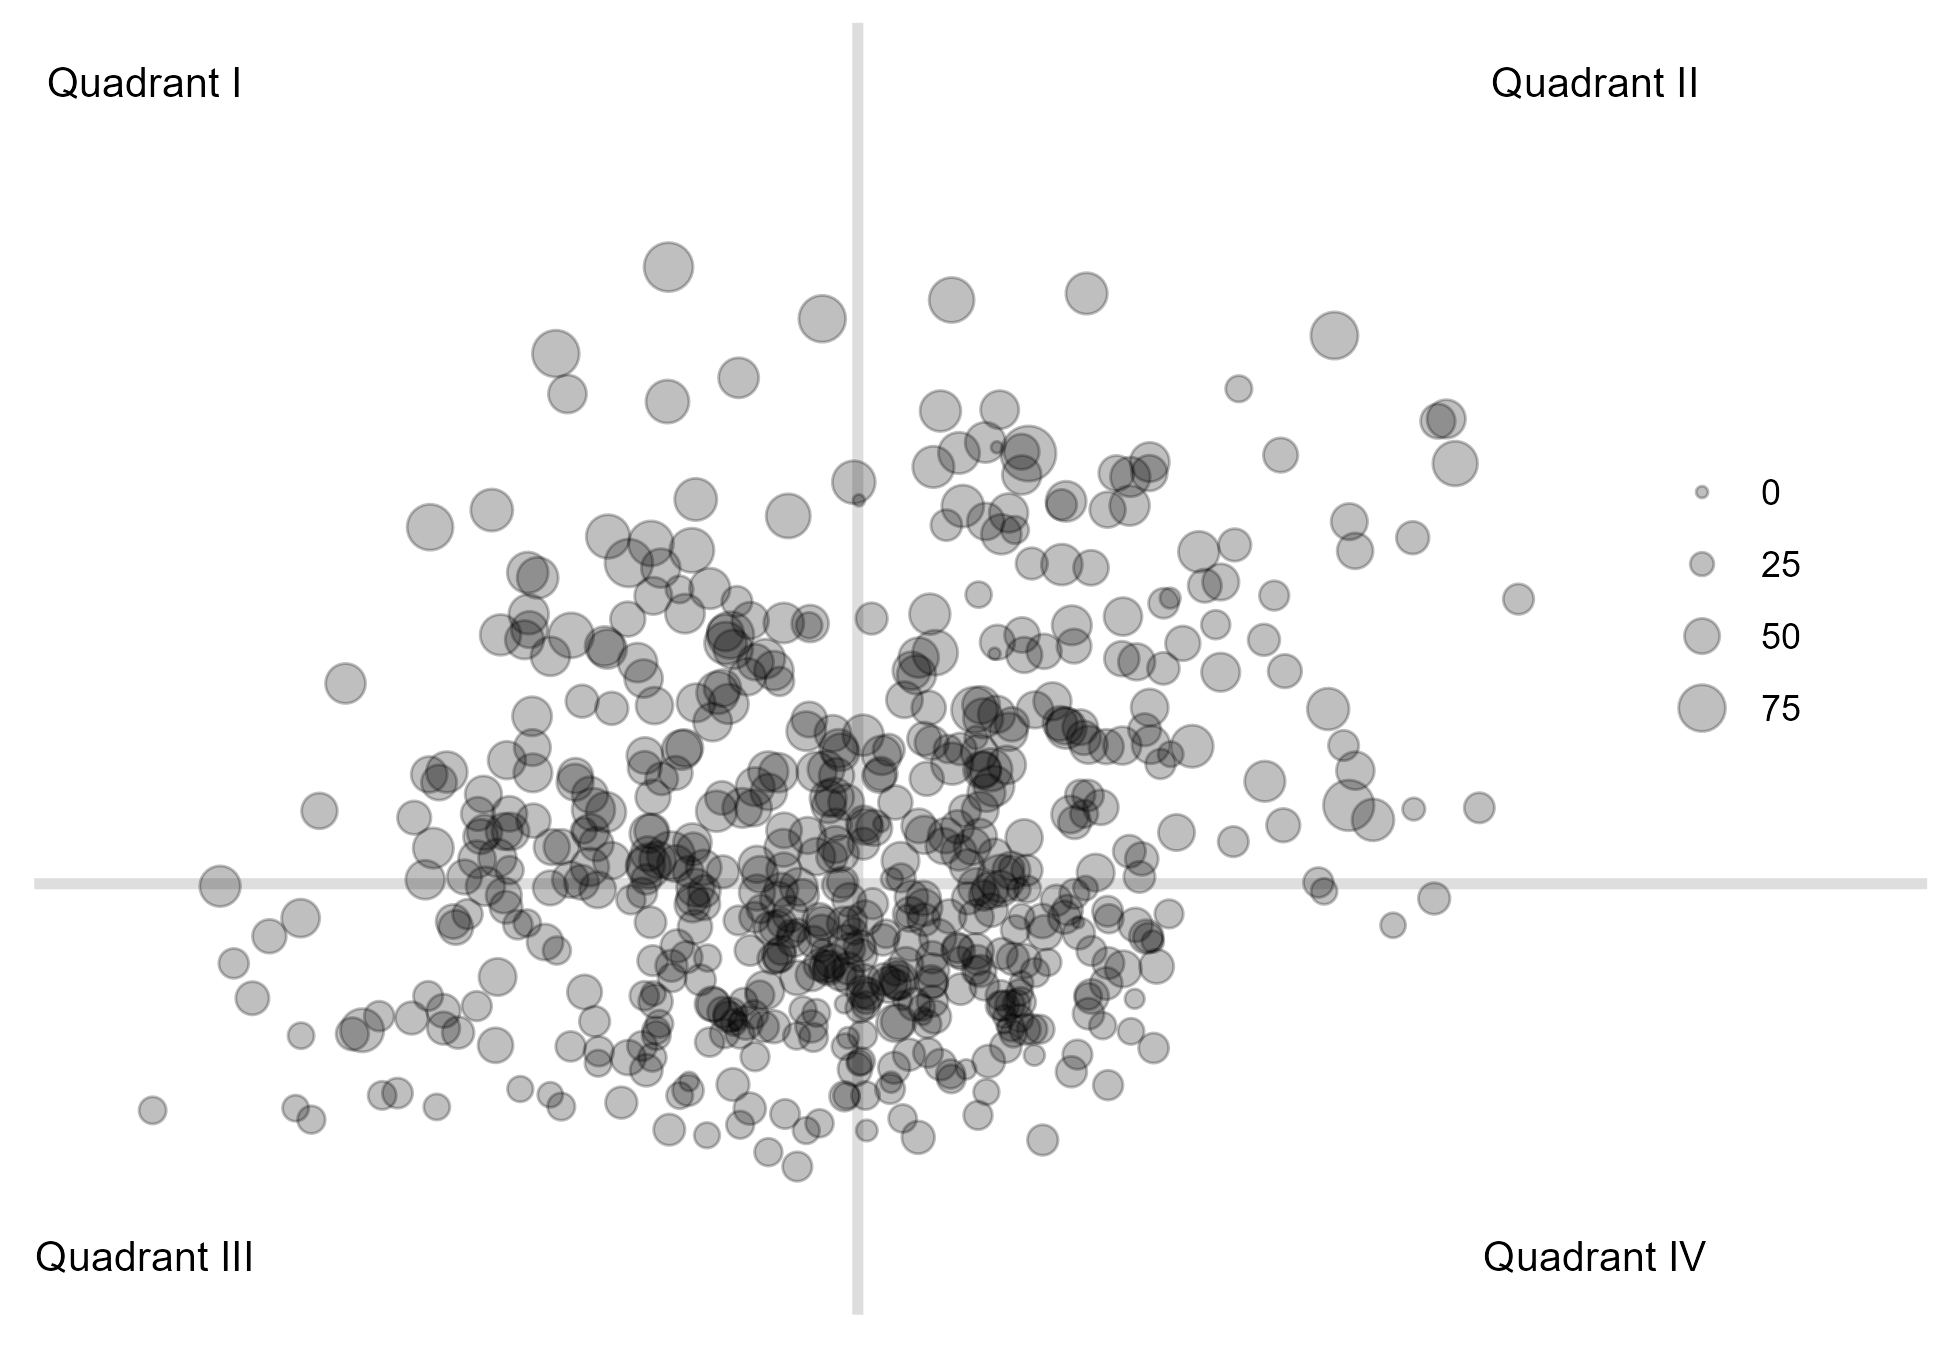
\includegraphics{figures/figure-1.png}
\caption{Vaccinations, Social Capital, and Personal Freedom}
\end{figure}

To provide a more quantitative assessment of our hypotheses, we develop
the following model, which specifies the basic functional form between
the values people have for personal freedom and/or public health and
their social capital:

\[
\begin{aligned}
Vaccination_{it}=\gamma_0+\gamma_1(Individual\ Values)_{i,t-7}+\gamma_2(Social\ Capital)_{i,t}+\\ \gamma_3(Individual\ Values_{i, t-7}*Social\ Capital_{i,t}) + v_{i,t}
\end{aligned}
\]

where we measure vaccination as the magnitude of vaccination, i.e., the
percentage of a county vaccinated on November 30, 2021. As of that date
people had had about 10-11 months to become vaccinated.\footnote{The FDA
  issued an EUA on Dec.~11, 2020 for the Pfizer vaccine.} This
vaccination data was collected from the Centers for Disease Control
(CDC) COVID-19 Vaccination Surveillance Database.

The interaction term between individual values and social capital allows
us to investigate our theoretical framework. That is, we can test the
following four hypotheses:

\begin{enumerate}
\def\labelenumi{\arabic{enumi}.}
\item
  Do counties that have a higher desire for public health have higher
  vaccination rates?
\item
  Do counties that have stronger measured social capital scores have
  more desire to protect their ``connections'' and, thus, higher
  vaccination rates?
\item
  Do counties with higher social capital and higher values for public
  health have higher vaccination rates?
\item
  Do counties with higher social capital and higher values for personal
  freedom have lower vaccination rates?
\end{enumerate}

Table 2 provides the descriptive statistics of these variables for our
sample dataset of 3,139 county-level observations.

\begin{table}[!htbp] \centering 
  \caption{} 
  \label{} 
\begin{tabular}{@{\extracolsep{5pt}}lcccccc} 
\\[-1.8ex]\hline 
\hline \\[-1.8ex] 
Statistic & \multicolumn{1}{c}{N} & \multicolumn{1}{c}{Min} & \multicolumn{1}{c}{Max} & \multicolumn{1}{c}{Mean} & \multicolumn{1}{c}{Median} & \multicolumn{1}{c}{St. Dev.} \\ 
\hline \\[-1.8ex] 
\% Vaccinated & 3,126 & 1.40 & 99.90 & 45.30 & 45.00 & 12.40 \\ 
Bar Days & 3,100 & 0 & 291 & 91.60 & 69 & 62.30 \\ 
Gathering Days & 3,099 & 0 & 296 & 206.00 & 269 & 102.00 \\ 
Mask Days & 3,100 & 0 & 266 & 132.00 & 169 & 90.30 \\ 
Restaurant Days & 3,100 & 0 & 131 & 53.80 & 52 & 20.40 \\ 
Stay at Home Days & 3,100 & 0 & 285 & 49.60 & 35 & 68.50 \\ 
Stringency & 3,099 & 0 & 1,003 & 533.00 & 599 & 229.00 \\ 
County Level Index & 2,960 & $-$4.32 & 2.97 & 0.005 & 0.004 & 1.00 \\ 
\% Republican & 3,099 & 8.73 & 96.20 & 65.10 & 68.40 & 16.00 \\ 
\% Bachelor's & 3,100 & 4.90 & 80.20 & 20.80 & 18.50 & 9.12 \\ 
\% Fair/Poor Health & 3,041 & 7.88 & 42.40 & 17.10 & 16.20 & 4.80 \\ 
\% Black & 3,100 & 0.00 & 86.20 & 8.98 & 2.15 & 14.50 \\ 
\% Rural & 3,100 & 0.00 & 100.00 & 58.50 & 59.40 & 31.40 \\ 
\% > 65 & 3,100 & 5.90 & 57.30 & 17.40 & 17.00 & 4.41 \\ 
Median Household Income & 3,099 & 18,972 & 125,672 & 47,817.00 & 46,227 & 12,498.00 \\ 
\hline \\[-1.8ex] 
\end{tabular} 
\end{table}

Table 3 presents results for the basic model and subsequent
specifications, where the dependent variable is the magnitude of
vaccination, i.e., the percentage of county population vaccinated on
November 30, 2021.

\begin{table}[!htbp] \centering 
  \caption{Regression Results} 
  \label{} 
\begin{tabular}{@{\extracolsep{5pt}}lcccc} 
\\[-1.8ex]\hline 
\hline \\[-1.8ex] 
 & \multicolumn{4}{c}{\textit{Dependent variable:}} \\ 
\cline{2-5} 
\\[-1.8ex] & \multicolumn{4}{c}{Percentage of County Vaccinated} \\ 
\\[-1.8ex] & (1) & (2) & (3) & (4)\\ 
\hline \\[-1.8ex] 
 Constant & 39.900$^{***}$ & 78.700$^{***}$ & 78.300$^{***}$ & 48.300$^{***}$ \\ 
  & (0.494) & (0.875) & (1.050) & (13.400) \\ 
  & & & & \\ 
 Public Health & 0.010$^{***}$ &  & 0.0004 & 0.040$^{***}$ \\ 
  & (0.001) &  & (0.001) & (0.016) \\ 
  & & & & \\ 
 Personal Freedom &  & $-$0.510$^{***}$ & $-$0.507$^{***}$ & $-$0.345$^{***}$ \\ 
  &  & (0.013) & (0.013) & (0.083) \\ 
  & & & & \\ 
 Social K & 0.213 & 7.400$^{***}$ & 6.100$^{***}$ & 3.850 \\ 
  & (0.486) & (0.749) & (0.844) & (15.000) \\ 
  & & & & \\ 
 Social K * Public Health & 0.003$^{***}$ &  & 0.002$^{**}$ & 0.038$^{**}$ \\ 
  & (0.001) &  & (0.001) & (0.017) \\ 
  & & & & \\ 
 Social K * Personal Freedom &  & $-$0.068$^{***}$ & $-$0.060$^{***}$ & $-$0.315$^{***}$ \\ 
  &  & (0.011) & (0.011) & (0.120) \\ 
  & & & & \\ 
\hline \\[-1.8ex] 
Observations & 2959 & 2959 & 2958 & 2935 \\ 
R2 & 0.053 & 0.418 & 0.42 &  \\ 
F Statistic & 54.9*** & 708.8*** & 426.7*** & 91.2*** \\ 
\hline 
\hline \\[-1.8ex] 
Standard errors are heteroskedasticity robust. & \multicolumn{4}{r}{$^{*}$p$<$0.1; $^{**}$p$<$0.05; $^{***}$p$<$0.01} \\ 
\end{tabular} 
\end{table}

Model 1 estimates equation 1 where individual values are the values for
public health; Model 2 estimates equation 1 where individual values are
the values for personal freedom; Model 3 estimates equation 1 with both
measures of individual values; and Model 4 uses an instrumental variable
technique.

All four regressions show statistically significant results and support
our initial propositions. Model 1 in Table 3 shows that a one unit
increase in the value for public health increases the magnitude of
vaccination by 0.01\%. The interaction between values for public health
and social capital increases the magnitude of vaccination by 0.003\%.
Model 2 shows that a one unit increase in the value for personal freedom
decreases the magnitude of vaccination by 0.51\%. A one standard
deviation increase in social capital increases the magnitude of
vaccination by 7.4\%. The interaction between the value for personal
freedom and social capital decreases the magnitude of vaccination by
0.07\%. Model 3 of Table 3 specifies the basic model with both measures
of individual values, along with both interaction effects. A one unit
increase in the values for personal freedom decreases the magnitude of
vaccination by 0.51\%. A one standard deviation increase in social
capital increases the magnitude of vaccination by 6.1\%. Moreover, the
interaction terms of Model 3 of Table 3 have the expected effect and are
statistically significant. The interaction term between social capital
and values for public health increases the magnitude of vaccination by
0.002\%, and the interaction term between social capital and values for
personal freedom decreases the magnitude of vaccination by 0.06\%. These
results suggest that social capital on net reinforces our values for
public health and personal freedom, respectively.

Model 3 likely suffers from endogeneity as the values for public health
and personal freedom depend on various demographic factors. With data
from the US Census American Community Survey (2019), the Bureau of
Economic Analysis, and the Bureau of Labor Statistics, we use the
following variables to instrument for the values for public health and
personal freedom: median family income, percent with a bachelor's
degree, percent black, percent in poor/fair health, percent rural, and
percent over 65. Our results suggest significant endogeneity. Model 4
shows the instrumental variable specification for model 3.

Model 4 appears to be a better specification for the relationship
between our main variables of interest.\footnote{The Wu-Hausmann test
  for weak instruments supports these results, which suggests our
  included variables are appropriate instruments.} Moreover, Model 4
shows results that are consistent with the general implication of our
previous models and provide a more robust analysis. A one unit increase
in the value for public health increases the magnitude of vaccination by
0.04\%. A one unit increase in the value for personal freedom decreases
the magnitude of vaccination by 0.35\%. The interaction between values
for public health and social capital increases the magnitude of
vaccination by 0.04\%, whereas the interaction between values for
personal freedom and social capital decreases the magnitude of
vaccination by 0.32\%.

Our results lend support for the social capital framework discussed
above. In particular, it suggests that social capital has an ambiguous
effect on vaccination rates. However, the level of social capital
mediates the normative values people have and can amplify those values.
Whereas people who value public health---and are more willing to use
stringent public health measures---use higher levels of social capital
to increase their magnitude of vaccination, people who value personal
freedom---and who might be more hesitant towards public health---use
higher levels of social capital to decrease their magnitude of
vaccination.

\hypertarget{robustness-check}{%
\section{Robustness Check}\label{robustness-check}}

As Ferwana and Varshney (2021) suggests, the effect social capital might
have on vaccination rates might vary depending a particular sub
component used in its construction. Table 4 shows whether these sub
components alone have a similar effect on the magnitude of vaccination.
We analyze these components using our baseline specifications found in
Model 1-3 of Table 3.

\begin{table}[!htbp] \centering 
  \caption{Regression Results} 
  \label{} 
\begin{tabular}{@{\extracolsep{5pt}}lccc} 
\\[-1.8ex]\hline 
\hline \\[-1.8ex] 
 & \multicolumn{3}{c}{\textit{Dependent variable:}} \\ 
\cline{2-4} 
\\[-1.8ex] & \multicolumn{3}{c}{Percentage of County Vaccinated} \\ 
\\[-1.8ex] & (1) & (2) & (3)\\ 
\hline \\[-1.8ex] 
 Constant & 39.600$^{***}$ & 81.700$^{***}$ & 82.100$^{***}$ \\ 
  & (0.501) & (0.986) & (1.230) \\ 
  & & & \\ 
 Public Health & 0.011$^{***}$ &  & $-$0.0005 \\ 
  & (0.001) &  & (0.001) \\ 
  & & & \\ 
 Personal Freedom &  & $-$0.548$^{***}$ & $-$0.550$^{***}$ \\ 
  &  & (0.014) & (0.015) \\ 
  & & & \\ 
 Family Unit & $-$2.150$^{***}$ & 10.100$^{***}$ & 9.250$^{***}$ \\ 
  & (0.642) & (0.771) & (0.945) \\ 
  & & & \\ 
 Community Health & $-$0.543 & 0.304 & $-$2.410 \\ 
  & (0.685) & (1.250) & (1.490) \\ 
  & & & \\ 
 Institutional Health & 4.960$^{***}$ & $-$3.790$^{***}$ & $-$2.890$^{**}$ \\ 
  & (0.603) & (0.953) & (1.180) \\ 
  & & & \\ 
 Collective Efficacy & $-$1.560$^{**}$ & 0.609 & $-$0.334 \\ 
  & (0.604) & (0.708) & (0.741) \\ 
  & & & \\ 
 Family Unit * Public Health & 0.005$^{***}$ &  & 0.001 \\ 
  & (0.001) &  & (0.001) \\ 
  & & & \\ 
 Community Health * Public Health & 0.001 &  & 0.003$^{***}$ \\ 
  & (0.001) &  & (0.001) \\ 
  & & & \\ 
 Institutional Health * Public Health & $-$0.004$^{***}$ &  & $-$0.001 \\ 
  & (0.001) &  & (0.001) \\ 
  & & & \\ 
 Collective Efficacy * Public Health & 0.0002 &  & 0.002$^{**}$ \\ 
  & (0.001) &  & (0.001) \\ 
  & & & \\ 
 Family Unit * Personal Freedom &  & $-$0.117$^{***}$ & $-$0.114$^{***}$ \\ 
  &  & (0.012) & (0.012) \\ 
  & & & \\ 
 Community Health * Personal Freedom &  & 0.012 & 0.030 \\ 
  &  & (0.017) & (0.018) \\ 
  & & & \\ 
 Institutional Health * Personal Freedom &  & 0.057$^{***}$ & 0.054$^{***}$ \\ 
  &  & (0.014) & (0.015) \\ 
  & & & \\ 
 Collective Efficacy * Personal Freedom &  & 0.001 & 0.004 \\ 
  &  & (0.011) & (0.010) \\ 
  & & & \\ 
\hline \\[-1.8ex] 
Observations & 2875 & 2875 & 2874 \\ 
R2 & 0.11 & 0.456 & 0.461 \\ 
F Statistic & 39.3*** & 266.8*** & 174.3*** \\ 
\hline 
\hline \\[-1.8ex] 
Standard errors are heteroskedasticity robust. & \multicolumn{3}{r}{$^{*}$p$<$0.1; $^{**}$p$<$0.05; $^{***}$p$<$0.01} \\ 
\end{tabular} 
\end{table}

As we disaggregate social capital, personal freedom remains
statistically significant and negative; a one unit increase in the value
for personal freedom decreases the magnitude of vaccination by 0.55. The
family unit and institutional health sub components are statistically
significant; in Models 2 and 3 a one standard deviation increase in the
family unit sub component increases the magnitude of vaccination by
9.2\%-10.1\% whereas a one standard deviation increase in the
institutional health sub component decreases the magnitude of
vaccination.

The interaction terms between the values for public health and personal
freedom and the measured sub components also show statistically
significant results. For example, a one unit increase in the interaction
between community health and the values for public health increases the
magnitude of vaccination by 0.003\% and a one unit increase in the
interaction between collective efficacy and the values for public health
increases the magnitude of vaccination by 0.002\%. A one unit increase
in the interaction between family unit and the values for personal
freedom decreases the magnitude of vaccinations by 0.11\%, and a one
unit increase in the interaction between institutional health and the
values for personal freedom increases the magnitude of vaccination by
0.05\%. These results are similar to Ferwana and Varshney (2021) which
finds that institutional health positively influences vaccination rates.

\hypertarget{discussion-and-conclusion}{%
\section{Discussion and Conclusion}\label{discussion-and-conclusion}}

Our framework and results show that the normative values people hold and
their formal and informal rules influence vaccine hesitancy.
Specifically, we formally analyze how the interaction between the values
people have for personal freedom over public health and their social
capital influences the magnitude of COVID-19 vaccinations. As we use
different proxies for the values people have and multiple
specifications, we find suggestive evidence for our three main
propositions: 1) counties where people have a larger value for public
health experience more vaccinations, 2) counties where people have a
higher level of social capital experience more vaccinations, 3) counties
where people have both a higher level of social capital and a higher
value for public health experience more vaccination, and 4) counties
where people have both a higher level of social capital and a higher
value for personal freedom experience less vaccination. Thus, we find
that social capital mediates the values people have and encourages
behaviors they find valuable; this might or might not encourage
vaccinations and/or improvements in public health.

We suggest that disease prevention policies focusing primarily on
formal, stringent measures are misguided when planners ignore social
capital and the values people hold dear. Stringent measures are less
effective when people have higher levels of social capital and when they
value public health. Moreover, stringent measures might be a source of
tension and less effective when people have higher levels of social
capital and when they value personal freedom.

While we show the interaction between social capital and the value
people have for public health, there are no clear policy levers. No one
person or group has the ability to alter social capital, change the
values people have for personal freedom over public health, or maintain
the effectiveness of stringent policies given individual values. Social
capital emerges when individuals value participating in social
interactions; it is not clear how governmental officials, let alone
public health officials, can know or can influence such values and
interactions. Even if officials could alter social capital, our results
suggest such policies would be effective only when people already value
prevention specifically and public health more generally.

\newpage

References

\hypertarget{refs}{}
\begin{CSLReferences}{1}{0}
\leavevmode\vadjust pre{\hypertarget{ref-adolph_pandemic_2021}{}}%
Adolph, Christopher, Kenya Amano, Bree Bang-Jensen, Nancy Fullman, and
John Wilkerson. 2021. {``Pandemic {Politics}: {Timing} {State}-{Level}
{Social} {Distancing} {Responses} to {COVID}-19.''} \emph{Journal of
Health Politics, Policy and Law} 46 (2): 211--33.
\url{https://doi.org/10.1215/03616878-8802162}.

\leavevmode\vadjust pre{\hypertarget{ref-aw_covid-19_2021}{}}%
Aw, Junjie, Jun Jie Benjamin Seng, Sharna Si Ying Seah, and Lian Leng
Low. 2021. {``{COVID}-19 {Vaccine} {Hesitancy}-{A} {Scoping} {Review} of
{Literature} in {High}-{Income} {Countries}.''} \emph{Vaccines} 9 (8):
900. \url{https://doi.org/10.3390/vaccines9080900}.

\leavevmode\vadjust pre{\hypertarget{ref-baccini_explaining_2021}{}}%
Baccini, Leonardo, and Abel Brodeur. 2021. {``Explaining {Governors}'
{Response} to the {COVID}-19 {Pandemic} in the {United} {States}.''}
\emph{American Politics Research} 49 (2): 215--20.
\url{https://doi.org/10.1177/1532673X20973453}.

\leavevmode\vadjust pre{\hypertarget{ref-borgonovi_evolution_2021}{}}%
Borgonovi, Francesca, Elodie Andrieu, and S. V. Subramanian. 2021.
{``The Evolution of the Association Between Community Level Social
Capital and {COVID}-19 Deaths and Hospitalizations in the {United}
{States}.''} \emph{Social Science \& Medicine (1982)} 278 (June):
113948. \url{https://doi.org/10.1016/j.socscimed.2021.113948}.

\leavevmode\vadjust pre{\hypertarget{ref-brennan_explaining_2016}{}}%
Brennan, Geoffrey, Lina Eriksson, Robert E. Goodin, and Nicholas
Southwood. 2016. \emph{Explaining {Norms}}. Illustrated edition. Oxford
New York: Oxford University Press.

\leavevmode\vadjust pre{\hypertarget{ref-cadeddu_understanding_2021}{}}%
Cadeddu, Chiara, Carolina Castagna, Martina Sapienza, Teresa Eleonora
Lanza, Rosaria Messina, Manuela Chiavarini, Walter Ricciardi, and Chiara
de Waure. 2021. {``Understanding the Determinants of Vaccine Hesitancy
and Vaccine Confidence Among Adolescents: A Systematic Review.''}
\emph{Human Vaccines \& Immunotherapeutics} 0 (0): 1--17.
\url{https://doi.org/10.1080/21645515.2021.1961466}.

\leavevmode\vadjust pre{\hypertarget{ref-carson_covid_2021}{}}%
Carson, Byron, Justin P. Isaacs, and Anthony M. Carilli. 2021. {``Covid
{Alone}: {The} {Complementarity} {Between} {Social} {Capital} and
{Formal} {Public} {Health} {Rules} in the {United} {States}.''} \{SSRN\}
\{Scholarly\} \{Paper\} ID 3863619. Rochester, NY: Social Science
Research Network. \url{https://doi.org/10.2139/ssrn.3863619}.

\leavevmode\vadjust pre{\hypertarget{ref-chuang_social_2015}{}}%
Chuang, Ying-Chih, Ya-Li Huang, Kuo-Chien Tseng, Chia-Hsin Yen, and
Lin-hui Yang. 2015. {``Social Capital and Health-Protective Behavior
Intentions in an Influenza Pandemic.''} \emph{PloS One} 10 (4):
e0122970. \url{https://doi.org/10.1371/journal.pone.0122970}.

\leavevmode\vadjust pre{\hypertarget{ref-corcoran_christian_2021}{}}%
Corcoran, Katie E., Christopher P. Scheitle, and Bernard D. DiGregorio.
2021. {``Christian {Nationalism} and {COVID}-19 {Vaccine} {Hesitancy}
and {Uptake}.''} \emph{Vaccine}, October.
\url{https://doi.org/10.1016/j.vaccine.2021.09.074}.

\leavevmode\vadjust pre{\hypertarget{ref-dube_vaccine_2013}{}}%
Dubé, Eve, Caroline Laberge, Maryse Guay, Paul Bramadat, Réal Roy, and
Julie A. Bettinger. 2013. {``Vaccine Hesitancy.''} \emph{Human Vaccines
\& Immunotherapeutics} 9 (8): 1763--73.
\url{https://doi.org/10.4161/hv.24657}.

\leavevmode\vadjust pre{\hypertarget{ref-dutta_third_2021}{}}%
Dutta, Sunasir, Christos Makridis, and Hayagreeva Rao. 2021. {``Do
{Third} {Places} {Matter}?: {The} {Effects} of {Foot} {Traffic}
{Concentration} in {Gathering} {Places} on {Financial} {Distress} and
{Physical} {Health} in {Communities}.''} \{SSRN\} \{Scholarly\}
\{Paper\} ID 3927572. Rochester, NY: Social Science Research Network.
\url{https://doi.org/10.2139/ssrn.3927572}.

\leavevmode\vadjust pre{\hypertarget{ref-eskola_how_2015}{}}%
Eskola, Juhani, Philippe Duclos, Melanie Schuster, and Noni E.
MacDonald. 2015. {``How to Deal with Vaccine Hesitancy?''}
\emph{Vaccine}, {WHO} {Recommendations} {Regarding} {Vaccine}
{Hesitancy}, 33 (34): 4215--17.
\url{https://doi.org/10.1016/j.vaccine.2015.04.043}.

\leavevmode\vadjust pre{\hypertarget{ref-ferwana_social_2021}{}}%
Ferwana, Ibtihal, and Lav R. Varshney. 2021. {``Social Capital
Dimensions Are Differentially Associated with {COVID}-19 Vaccinations,
Masks, and Physical Distancing.''} \emph{PLOS ONE} 16 (12): e0260818.
\url{https://doi.org/10.1371/journal.pone.0260818}.

\leavevmode\vadjust pre{\hypertarget{ref-gopnik_paradoxical_2020}{}}%
Gopnik, Adam. 2020. {``The {Paradoxical} {Role} of {Social} {Capital} in
the {Coronavirus} {Pandemic}.''} \emph{The New Yorker}.
\url{https://www.newyorker.com/news/daily-comment/the-paradoxical-role-of-social-capital-in-the-coronavirus-pandemic}.

\leavevmode\vadjust pre{\hypertarget{ref-hildreth_targeting_2021}{}}%
Hildreth, James E. K., and Donald J. Alcendor. 2021. {``Targeting
{COVID}-19 {Vaccine} {Hesitancy} in {Minority} {Populations} in the
{US}: {Implications} for {Herd} {Immunity}.''} \emph{Vaccines} 9 (5):
489. \url{https://doi.org/10.3390/vaccines9050489}.

\leavevmode\vadjust pre{\hypertarget{ref-hudson_predictors_2021}{}}%
Hudson, Amanda, and William J. Montelpare. 2021. {``Predictors of
{Vaccine} {Hesitancy}: {Implications} for {COVID}-19 {Public} {Health}
{Messaging}.''} \emph{International Journal of Environmental Research
and Public Health} 18 (15): 8054.
\url{https://doi.org/10.3390/ijerph18158054}.

\leavevmode\vadjust pre{\hypertarget{ref-imbulana_arachchi_role_2021}{}}%
Imbulana Arachchi, Janaki, and Shunsuke Managi. 2021. {``The Role of
Social Capital in {COVID}-19 Deaths.''} \emph{BMC Public Health} 21 (1):
434. \url{https://doi.org/10.1186/s12889-021-10475-8}.

\leavevmode\vadjust pre{\hypertarget{ref-iwai-saito_social_2021}{}}%
Iwai-Saito, Kousuke, Yugo Shobugawa, and Katsunori Kondo. 2021.
{``Social Capital and Pneumococcal Vaccination ({Ppsv23}) in
Community-Dwelling Older {Japanese}: A {JAGES} Multilevel
Cross-Sectional Study.''} \emph{BMJ Open} 11 (6): e043723.
\url{https://doi.org/10.1136/bmjopen-2020-043723}.

\leavevmode\vadjust pre{\hypertarget{ref-jung_associations_2013}{}}%
Jung, Minsoo, Leesa Lin, and K. Viswanath. 2013. {``Associations Between
Health Communication Behaviors, Neighborhood Social Capital, Vaccine
Knowledge, and Parents' {H1n1} Vaccination of Their Children.''}
\emph{Vaccine} 31 (42): 4860--66.
\url{https://doi.org/10.1016/j.vaccine.2013.07.068}.

\leavevmode\vadjust pre{\hypertarget{ref-karafillakis_vaccine_2016}{}}%
Karafillakis, Emilie, Irina Dinca, Franklin Apfel, Sabrina Cecconi,
Andrea Wűrz, Judit Takacs, Jonathan Suk, Lucia Pastore Celentano, Piotr
Kramarz, and Heidi J. Larson. 2016. {``Vaccine Hesitancy Among
Healthcare Workers in {Europe}: {A} Qualitative Study.''} \emph{Vaccine}
34 (41): 5013--20. \url{https://doi.org/10.1016/j.vaccine.2016.08.029}.

\leavevmode\vadjust pre{\hypertarget{ref-khubchandani_covid-19_2021}{}}%
Khubchandani, Jagdish, and Yilda Macias. 2021. {``{COVID}-19 Vaccination
Hesitancy in {Hispanics} and {African}-{Americans}: {A} Review and
Recommendations for Practice.''} \emph{Brain, Behavior, \& Immunity -
Health} 15 (August): 100277.
\url{https://doi.org/10.1016/j.bbih.2021.100277}.

\leavevmode\vadjust pre{\hypertarget{ref-larson_understanding_2014}{}}%
Larson, Heidi J., Caitlin Jarrett, Elisabeth Eckersberger, David M. D.
Smith, and Pauline Paterson. 2014. {``Understanding Vaccine Hesitancy
Around Vaccines and Vaccination from a Global Perspective: {A}
Systematic Review of Published Literature, 2007--2012.''} \emph{Vaccine}
32 (19): 2150--59. \url{https://doi.org/10.1016/j.vaccine.2014.01.081}.

\leavevmode\vadjust pre{\hypertarget{ref-lazarus_hesitant_2020}{}}%
Lazarus, Jeffrey V., Katarzyna Wyka, Lauren Rauh, Kenneth Rabin, Scott
Ratzan, Lawrence O. Gostin, Heidi J. Larson, and Ayman El-Mohandes.
2020. {``Hesitant or {Not}? {The} {Association} of {Age}, {Gender}, and
{Education} with {Potential} {Acceptance} of a {COVID}-19 {Vaccine}: {A}
{Country}-Level {Analysis}.''} \emph{Journal of Health Communication} 25
(10): 799--807. \url{https://doi.org/10.1080/10810730.2020.1868630}.

\leavevmode\vadjust pre{\hypertarget{ref-macdonald_vaccine_2015}{}}%
MacDonald, Noni E., and SAGE Working Group on Vaccine Hesitancy. 2015.
{``Vaccine Hesitancy: {Definition}, Scope and Determinants.''}
\emph{Vaccine} 33 (34): 4161--64.
\url{https://doi.org/10.1016/j.vaccine.2015.04.036}.

\leavevmode\vadjust pre{\hypertarget{ref-makridis_how_2021}{}}%
Makridis, Christos A., and Cary Wu. 2021. {``How Social Capital Helps
Communities Weather the {COVID}-19 Pandemic.''} \emph{PLOS ONE} 16 (1):
e0245135. \url{https://doi.org/10.1371/journal.pone.0245135}.

\leavevmode\vadjust pre{\hypertarget{ref-mollalo_spatial_2021}{}}%
Mollalo, Abolfazl, and Moosa Tatar. 2021. {``Spatial {Modeling} of
{COVID}-19 {Vaccine} {Hesitancy} in the {United} {States}.''}
\emph{International Journal of Environmental Research and Public Health}
18 (18): 9488. \url{https://doi.org/10.3390/ijerph18189488}.

\leavevmode\vadjust pre{\hypertarget{ref-nagaoka_income_2012}{}}%
Nagaoka, Kei, Takeo Fujiwara, and Jun Ito. 2012. {``Do Income Inequality
and Social Capital Associate with Measles-Containing Vaccine Coverage
Rate?''} \emph{Vaccine} 30 (52): 7481--88.
\url{https://doi.org/10.1016/j.vaccine.2012.10.055}.

\leavevmode\vadjust pre{\hypertarget{ref-nawa_association_2019}{}}%
Nawa, Nobutoshi, and Takeo Fujiwara. 2019. {``Association Between Social
Capital and Second Dose of Measles Vaccination in {Japan}: {Results}
from the {A}-{CHILD} Study.''} \emph{Vaccine} 37 (6): 877--81.
\url{https://doi.org/10.1016/j.vaccine.2018.12.037}.

\leavevmode\vadjust pre{\hypertarget{ref-ozawa_public_2013}{}}%
Ozawa, Sachiko, and Meghan L Stack. 2013. {``Public Trust and Vaccine
Acceptance-International Perspectives.''} \emph{Human Vaccines \&
Immunotherapeutics} 9 (8): 1774--78.
\url{https://doi.org/10.4161/hv.24961}.

\leavevmode\vadjust pre{\hypertarget{ref-pitas_social_2020}{}}%
Pitas, Nicholas, and Colin Ehmer. 2020. {``Social {Capital} in the
{Response} to {COVID}-19.''} \emph{American Journal of Health Promotion}
34 (8): 942--44.
\url{https://journals.sagepub.com/doi/full/10.1177/0890117120924531}.

\leavevmode\vadjust pre{\hypertarget{ref-putnam_bowling_2001}{}}%
Putnam, Robert D. 2001. \emph{Bowling {Alone}: {The} {Collapse} and
{Revival} of {American} {Community}}. Anniversary edition. Simon \&
Schuster.

\leavevmode\vadjust pre{\hypertarget{ref-ronnerstrand_social_2014}{}}%
Rönnerstrand, B. 2014. {``Social Capital and Immunization Against the
2009 {A}({H1N1}) Pandemic in the {American} {States}.''} \emph{Public
Health} 128 (8): 709--15.
\url{https://doi.org/10.1016/j.puhe.2014.05.015}.

\leavevmode\vadjust pre{\hypertarget{ref-ronnerstrand_social_2013}{}}%
Rönnerstrand, Björn. 2013. {``Social Capital and Immunisation Against
the 2009 {A}({H1N1}) Pandemic in {Sweden}.''} \emph{Scandinavian Journal
of Public Health} 41 (8): 853--59.
\url{https://doi.org/10.1177/1403494813494975}.

\leavevmode\vadjust pre{\hypertarget{ref-wong_social_2020}{}}%
Wong, Anna S. Y., and Jillian C. Kohler. 2020. {``Social Capital and
Public Health: Responding to the {COVID}-19 Pandemic.''}
\emph{Globalization and Health} 16 (1): 88.
\url{https://doi.org/10.1186/s12992-020-00615-x}.

\leavevmode\vadjust pre{\hypertarget{ref-xiao_vaccine_2020}{}}%
Xiao, Xizhu, and Rachel Min Wong. 2020. {``Vaccine Hesitancy and
Perceived Behavioral Control: {A} Meta-Analysis.''} \emph{Vaccine} 38
(33): 5131--38. \url{https://doi.org/10.1016/j.vaccine.2020.04.076}.

\leavevmode\vadjust pre{\hypertarget{ref-yaqub_attitudes_2014}{}}%
Yaqub, Ohid, Sophie Castle-Clarke, Nick Sevdalis, and Joanna Chataway.
2014. {``Attitudes to Vaccination: {A} Critical Review.''} \emph{Social
Science \& Medicine} 112 (July): 1--11.
\url{https://doi.org/10.1016/j.socscimed.2014.04.018}.

\end{CSLReferences}

\end{document}
